\documentclass[a4paper,10pt]{article}
\usepackage[utf8]{inputenc}

\usepackage[english]{babel}
\usepackage{xcolor}
\usepackage[compact,small]{titlesec}
\usepackage{booktabs}
\usepackage{multirow}
\usepackage{amsfonts,amsmath,amssymb}
\usepackage{marginnote}
\usepackage[top=1.8cm, bottom=1.8cm, outer=1.8cm, inner=1.8cm, heightrounded, marginparwidth=2.5cm, marginparsep=0.5cm]{geometry}
\usepackage{enumitem}
\setlist{noitemsep,parsep=2pt}
\newcommand{\highlight}[1]{\textcolor{kuleuven}{#1}}
\usepackage{pythonhighlight}
\usepackage{cleveref}
\usepackage{graphicx}

\usepackage{tikz}

\def\retake{0}
\newcommand{\switch}[2]{\ifnum\retake=0{#1}\else{#2}\fi}


\newcommand{\nextyear}{\advance\year by 1 \the\year\advance\year by -1}
\newcommand{\thisyear}{\the\year}
\newcommand{\deadlineCode}{\switch{December 28, \thisyear{} at 9:00 CET}{August 4, \thisyear{} at 9:00 CET}}
\newcommand{\deadlineReport}{\deadlineCode}

\newcommand{\ReplaceMe}[1]{{\color{blue}#1}}
\newcommand{\RemoveMe}[1]{{\color{purple}#1}}

\setlength{\parskip}{5pt}

%opening
\title{\vspace{-2cm}Evolutionary Algorithms: \switch{Final}{Retake} report}
\author{\ReplaceMe{Your Name (r0123456)}}

\begin{document}
\fontfamily{ppl}
\selectfont{}

\maketitle

\RemoveMe{
\section*{Formal requirements} \label{sec_this}

The report is structured for fair and efficient grading of around 100 individual projects in the space of only a few days. Please respect the exact structure of this document. You are allowed to remove this section and \cref{sec_other}. Brevity is the soul of wit: a good report will be \textbf{around $8$ pages} long. The hard limit is 10 pages. 
This \textbf{excludes} the other comments in \cref{sec_other} and the generative AI compliance form in \cref{sec_genai}, which have no page limit.

\begin{quote}
Think of this report as a \textbf{take-home exam}; it will be used at the exam for structuring the discussion and questions. Make an effort so that it can be visually scanned efficiently, e.g., by using boldface or colors to highlight key points, using lists, clearly defined paragraphs, figures, etc.

You do not need to explain in this report \textbf{how} the techniques and concepts that are literally in the slides work. The goal of this report is \textbf{not} to illustrate that you can reproduce the slides. You need to convince me that you aptly used these (and other) techniques in this project. If I have doubts about your understanding of certain concepts in the course materials, I will test this hypothesis at the exam.
\end{quote}

It is recommended that you use this \LaTeX{} template, but you are allowed to reproduce it with the same structure in a WYSIWYG-editor. The purple text containing our evaluation criteria can be removed. You should replace the blue text with your discussion.

This report should be uploaded to Toledo by \deadlineReport. It must be in the \textbf{Portable Document Format} (pdf) and must be named \texttt{r0123456\_final.pdf}, where r0123456 should be replaced with your student number.

Remove the current section from your final report.
}

\section{Metadata}

\begin{itemize}
 \item \textbf{Group members during group phase:} \ReplaceMe{Group member 1} and \ReplaceMe{group member 2}
 \item \textbf{Time spent on group phase:} \ReplaceMe{10 hours}
 \item \textbf{Time spent on final code:} \ReplaceMe{40 hours}
 \item \textbf{Time spent on final report:} \ReplaceMe{10 hours}
\end{itemize}

\section{Changes since \switch{the group phase}{your previous submission} \hfill(target: $0.25$ pages)}

\ReplaceMe{List the main changes that you implemented since \switch{the group phase}{your previous submission of the project}. You do not need to explain the employed techniques in detail; for this, you should refer to the appropriate subsection of section 3 of the report.}

\begin{enumerate}
 \item \ReplaceMe{State here the modification that you made (e.g., replaced top-$\lambda$ selection with $k$-tournament selection).}
 \item \dots
\end{enumerate}

\section{Final design of the evolutionary algorithm \hfill(target: $3.5$ pages)} 

\RemoveMe{\textbf{Goal:} Based on this section, we will evaluate insofar as you are able to design and implement an advanced, effective evolutionary algorithm for solving a model problem.}


\subsection{The three main features}
\ReplaceMe{List the three main components of your evolutionary algorithm for this project. That is, what are its most distinctive characteristics, what components am I not allowed to change to a more basic version? Ideally these are some of the more advanced features that you added since \switch{the group phase}{your previous submission}.}

\begin{enumerate}
 \item \ReplaceMe{Just state the feature, you do not need to explain it, instead refer to the appropriate section below.}
 \item \dots
 \item \dots
\end{enumerate}

\subsection{The main loop}

\ReplaceMe{Make a picture of the ``flow'' in your evolutionary algorithm, similar to the example below. Include all the main components (mutation, recombination, selection, elimination, initialization, local search operators, diversity promotion mechanisms). There are no formal requirements on how to do this, as long as it is clear and you can efficiently explain your complete evolutionary algorithm using this picture at the exam. Contrary to the picture below, include the specific techniques, e.g., top-$\lambda$ elimination, $k$-tournament selection, where possible.

\begin{center}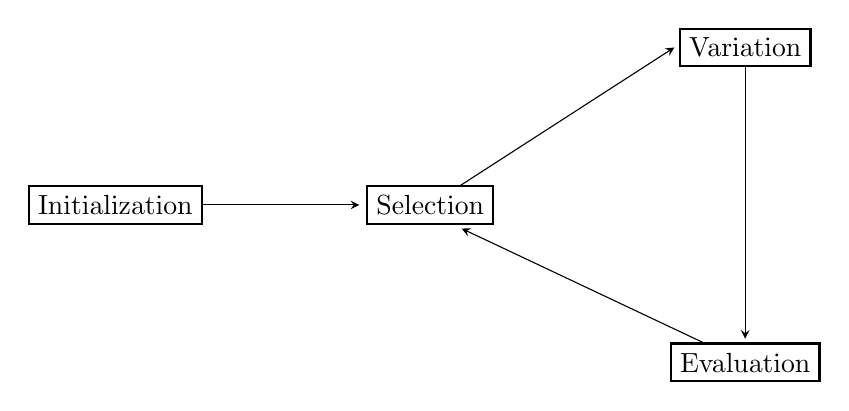
\begin{tikzpicture}
\draw[->,>=stealth] (0,0) -- (3.1,0);
\draw[->,>=stealth] (4,0) -- (7.1,2);
\draw[->,>=stealth] (8,2) -- (8,-1.7);
\draw[->,>=stealth] (8,-2) -- (4.4,-.3);
\node[draw,rectangle,thick,fill=white] at (0,0) {Initialization};
\node[draw,rectangle,thick,fill=white] at (4,0) {Selection};
\node[draw,rectangle,thick,fill=white] at (8,2) {Variation};
\node[draw,rectangle,thick,fill=white] at (8,-2) {Evaluation};
\end{tikzpicture}\end{center}
}

\RemoveMe{\textbf{The questions from \cref{sec_rep} to \cref{sec_oth} in blue are there to guide which topics to discuss}, rather than an exact list of questions that must be answered. Feel free to add more items to discuss.}

\subsection{Representation}\label{sec_rep}

\ReplaceMe{How do you represent the candidate solutions? What is your motivation to choose this one? What other options did you consider? How did you implement this specifically in Python (e.g., a list, set, numpy array, etc)?}

\subsection{Initialization}

\ReplaceMe{How do you initialize the population? How did you determine the number of individuals? Did you implement advanced initialization mechanisms (local search operators, heuristic solutions)? If so, describe them. Do you believe your approach maintains sufficient diversity? How do you ensure that your population enrichment scheme does not immediately take over the population? Did you implement other initialization schemes that did not make it to the final version? Why did you discard them? How did you determine the population size?}

\subsection{Selection operators}

\ReplaceMe{Which selection operators did you implement? If they are not from the slides, describe them. Can you motivate why you chose this one? Are there parameters that need to be chosen? Did you use an advanced scheme to vary these parameters throughout the iterations? Did you try other selection operators not included in the final version? Why did you discard them?}

\subsection{Mutation operators}

\ReplaceMe{Which mutation operators did you implement? If they are not from the slides, describe them. How do you choose among several mutation operators? Do you believe it will introduce sufficient randomness? Can that be controlled with parameters? Do you use self-adaptivity? Do you use any other advanced parameter control mechanisms (e.g., variable across iterations)? Did you try other mutation operators not included in the final version? Why did you discard them?}

\subsection{Recombination operators}

\ReplaceMe{Which recombination operators did you implement? If they are not from the slides, describe them. How do you choose among several recombination operators? Why did you choose these ones specifically? Explain how you believe that these operators can produce offspring that combine the best features from their parents. How does your operator behave if there is little overlap between the parents? Can your recombination be controlled with parameters; what behavior do they change? Do you use self-adaptivity? Do you use any other advanced parameter control mechanisms (e.g., variable across iterations)? Did you try other recombination operators not included in the final version? Why did you discard them? Did you consider recombination with arity strictly greater than 2?}

\subsection{Elimination operators}

\ReplaceMe{Which elimination operators did you implement? If they are not from the slides, describe them. Why did you select this one? Are there parameters that need to be chosen? Did you use an advanced scheme to vary these parameters throughout the iterations? Did you try other elimination operators not included in the final version? Why did you discard them?} 

\subsection{Local search operators}

\ReplaceMe{What local search operators did you implement? Describe them. Did they cause a significant improvement in the performance of your algorithm? Why (not)? Did you consider other local search operators that did not make the cut? Why did you discard them? Are there parameters that need to be determined in your operator? Do you use an advanced scheme to determine them (e.g., adaptive or self-adaptive)?}

\subsection{Diversity promotion mechanisms}

\ReplaceMe{Did you implement a diversity promotion scheme? If yes, which one? If no, why not? Describe the mechanism you implemented. In what sense does the mechanism improve the performance of your evolutionary algorithm? Are there parameters that need to be determined? Did you use an advanced scheme to determine them?}

\subsection{Stopping criterion}

\ReplaceMe{Which stopping criterion did you implement? Did you combine several criteria?}

\subsection{Parameter selection}

\ReplaceMe{For all of the parameters that are not automatically determined by adaptivity or self-adaptivity (as you have described above), describe how you determined them. Did you perform a hyperparameter search? How did you do this? How did you determine these parameters would be valid both for small and large problem instances?}

\subsection{Other considerations}\label{sec_oth}

\ReplaceMe{Did you consider other items not listed above, such as elitism, multiobjective optimization strategies (e.g., island model, pareto front approximation), a parallel implementation, or other interesting computational optimizations (e.g. using advanced algorithms or data structures)? You can describe them here or add additional subsections as needed.}


\section{Numerical experiments \hfill(target: 1.5 pages)}

\RemoveMe{\textbf{Goal:} Based on this section and our execution of your code, we will evaluate the performance (time, quality of solutions) of your implementation and your ability to interpret and explain the results on benchmark problems.}

\subsection{Metadata}

\ReplaceMe{What parameters are there to choose in your evolutionary algorithm? Which fixed parameter values did you use for all experiments below? If some parameters are determined based on information from the problem instance (e.g., number of cities), also report their specific values for the problems below.

Report the main characteristics of the computer system on which you ran your evolutionary algorithm. Include the processor or CPU (including the number of cores and clock speed), the amount of main memory, and the version of Python 3.}


\subsection{tour50.csv}

\ReplaceMe{Run your algorithm on this benchmark problem (with the 5 minute time limit from the Reporter). \textbf{Include a typical convergence graph, by plotting the mean and best objective values in function of the time} (for example based on the output of the Reporter class).

What is the best tour length you found? What is the corresponding sequence of cities? 

Interpret your results. How do you rate the performance of your algorithm (time, memory, speed of convergence, diversity of population, quality of the best solution, etc)? Is your solution close to the optimal one?

Solve this problem 500 times and record the results. Make a histogram of the final mean fitnessess and the final best fitnesses of the 500 runs. Comment on this figure: is there a lot of variability in the results, what are the means and the standard deviations?}

\subsection{tour250.csv}\label{sec_shorttour}
\ReplaceMe{Run your algorithm on this benchmark problem (with the 5 minute time limit from the Reporter). \textbf{Include a typical convergence graph, by plotting the mean and best objective values in function of the time} (for example based on the output of the Reporter class).

What is the best tour length you found in each case? 

Interpret your results. How do you rate the performance of your algorithm (time, memory, speed of convergence, diversity of population, quality of the best solution, etc)? Is your solution close to the optimal one?}


\subsection{tour1000.csv}

\ReplaceMe{Answer the same questions as in \cref{sec_shorttour}.}

\section{Critical reflection \hfill(target: $1.5$ page)}

\RemoveMe{\textbf{Goal:} Based on this section, we will evaluate your understanding and insight into the main strengths and weaknesses of evolutionary algorithms, as well as your insights into responsible genAI usage.}

\subsection{Strengths and weaknesses}
\ReplaceMe{What are the three main strengths of evolutionary algorithms in your experience?}

\begin{enumerate}
 \item 
 \item 
 \item 
\end{enumerate}

\ReplaceMe{What are the three main weak points of evolutionary algorithms in your experience?}

\begin{enumerate}
 \item 
 \item 
 \item 
\end{enumerate}

\ReplaceMe{Describe the main lessons learned from this project. Do you believe evolutionary algorithms are appropriate for the problem studied in this project? Why (not)? What surprised you and why? What did you learn from this project?}

\subsection{GenAI peer reviewing critical reflection} 
\ReplaceMe{What are the strengths and weaknesses of the AI-generated peer review compared to the human-written one? Did Copilot identify issues the humans missed, or vice versa? Why do you think this happened? Was Copilot's review at all useful? Was it specific and concrete or rather vague and general? What is your view towards reviewing reports using generative AI? Would you want to be reviewed by an AI system or by a human? Why? Did writing your own review help you understand the other group's algorithm better than reading the AI’s version? How might relying too much on AI affect your ability to critically evaluate scientific work in the future? In what ways can AI be a helpful tool in peer review? In what ways can it be harmful?}

\subsection{GenAI critical reflection}
\ReplaceMe{In what ways did generative AI help you during the project? In what ways did it hinder your learning or understanding?
Briefly describe for which activities you believe genAI added value:
\begin{enumerate}
 \item 
 \item
 \item
\end{enumerate}
For which activities did you not observe any or sufficient added value:
\begin{enumerate}
 \item 
 \item
 \item
\end{enumerate}
}

\ReplaceMe{Would your project solution have been substantially different without relying on genAI? In what aspects? Why? How much time did you gain or lose by relying on genAI? If you did not substantially employ genAI: motivate why did you not use it.}


\clearpage
\section{Other comments \hfill(does not count toward page limit)} \label{sec_other}

\ReplaceMe{In case there is something important to discuss that is not covered by the previous sections, you can do it here. }

\section{Generative AI compliance form \hfill(does not count toward page limit)} \label{sec_genai}

\RemoveMe{For \textbf{each instance} of a genAI activity that required reporting (generating ideas and code), fill out the following information. You do not need to provide this information for the unconditionally approved uses of genAI.}

\subsection{Example activity} \ReplaceMe{Briefly describe the activity for which you employed GenAI. For example: ``Code skeleton generation for a recombination operator of permutations.'' Give the subsection an informative title.}

\paragraph{Generative AI model:} \ReplaceMe{Identify the GenAI model used for this activity. For example, Microsoft Copilot, OpenAI ChatGPT v4, Midjourney, etc.}

\paragraph{Motivation:} \ReplaceMe{Describe the intention and reason for employing generative AI for this activity.}

\paragraph{Methodology:} \ReplaceMe{List the exact prompts you used to generate the content. You do not need to include the model's response.}

\paragraph{Postprocessing:} \ReplaceMe{Describe which postprocessing you applied to the generated content. For example, ``the output was used verbatim,'' ``the output contained basic programming errors (undefined variables, undefined functions), which I corrected by hand,'' ``I rewrote/removed/expanded one/a few/some/most/all sentences to [purpose],'' ``The generated content contained interesting ideas for a recombination operator, suggesting in particular to [do it in such and such way]. However, this idea would have been computationally very expensive, so I simplified [this and that], using [advanced data structure] to obtain an efficient variant of the generated idea.''}

\paragraph{Reflection:} \ReplaceMe{Critically reflect on the output generated and describe what you learned and in which aspects the result was useful and in which aspects it was not useful.}


\subsection{Another example activity} 
\paragraph{Generative AI model:}
\paragraph{Motivation:}
\paragraph{Methodology:}
\paragraph{Postprocessing:}
\paragraph{Reflection:} 

\end{document}
